\chapter{Product CAD \& Electrical Diagrams}

\section{Structures CAD}
3D CAD images as well as dimensioned engineering drawings of the structural components of the project are shown in Figures \ref{cad:arm} through \ref{cad:track:dwg}.

\begin{figure}[H]
    \centering
    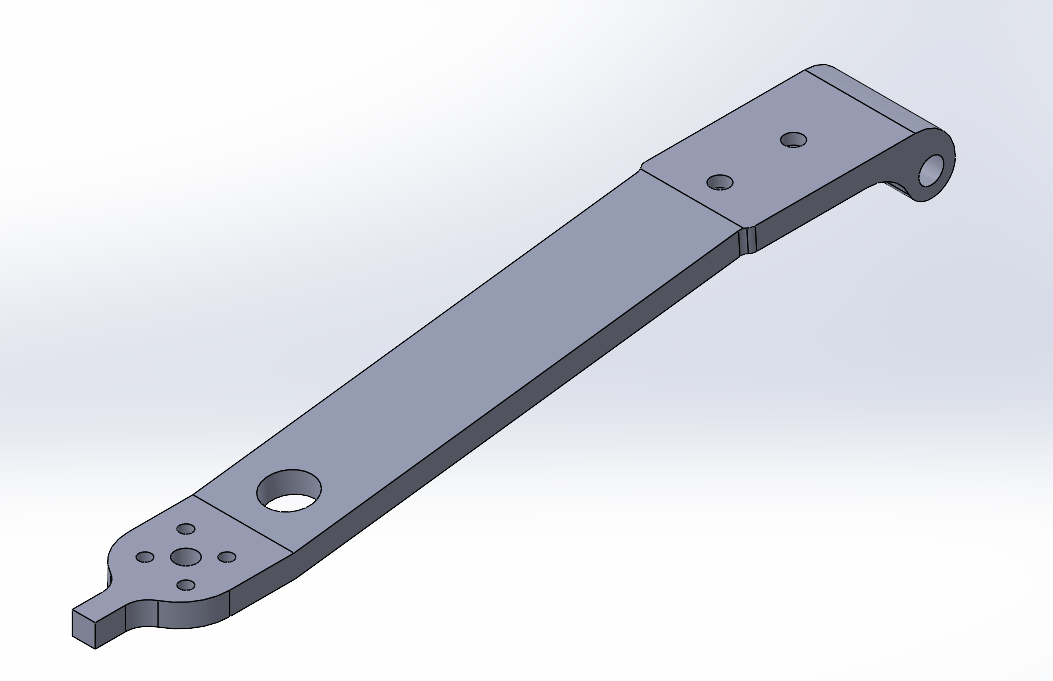
\includegraphics[width=0.7\textwidth]{src/figs/arm-cad.png}
    \caption{Arm}
    \label{cad:arm}
\end{figure}

\begin{figure}[H]
    \centering
    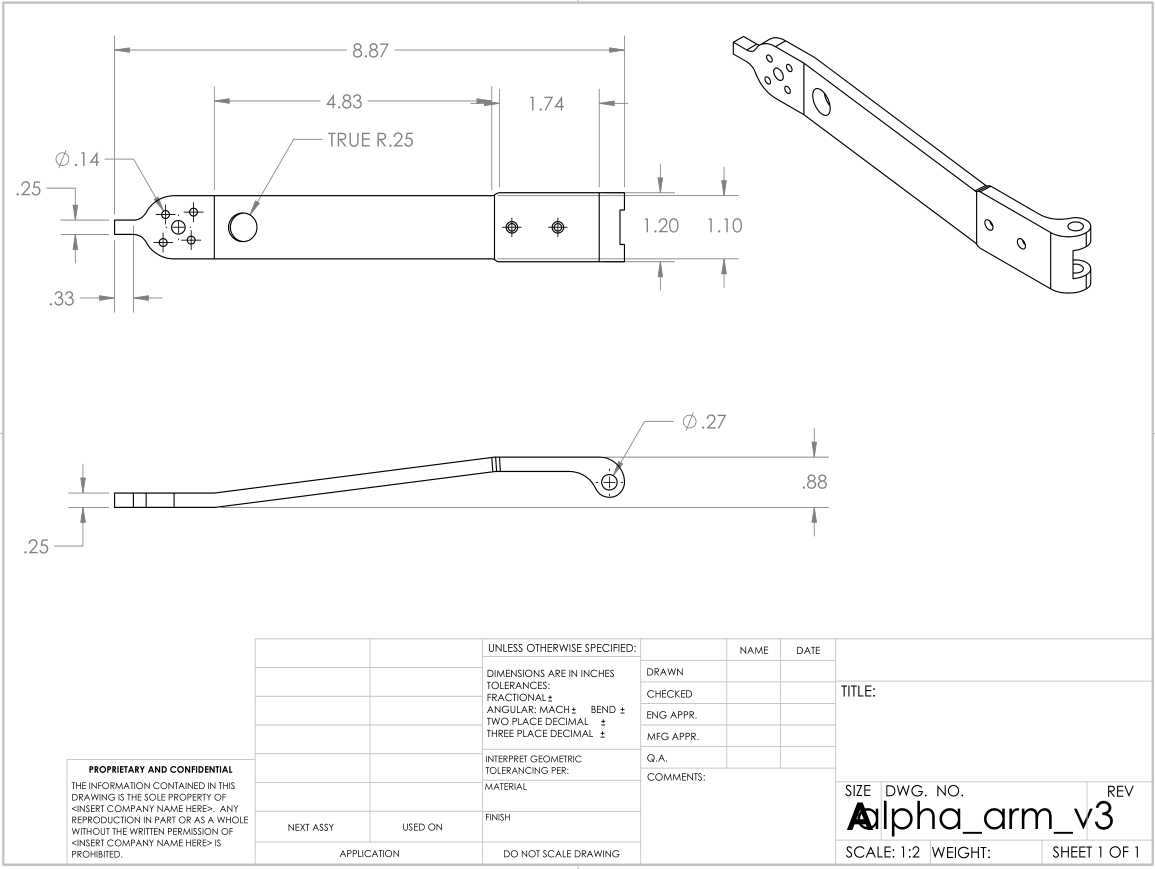
\includegraphics[width=\textwidth]{src/figs/cad-and-dwgs/arm_dwg.png}
    \caption{Arm drawing}
    \label{cad:arm:dwg}
\end{figure}

\begin{figure}[H]
    \centering
    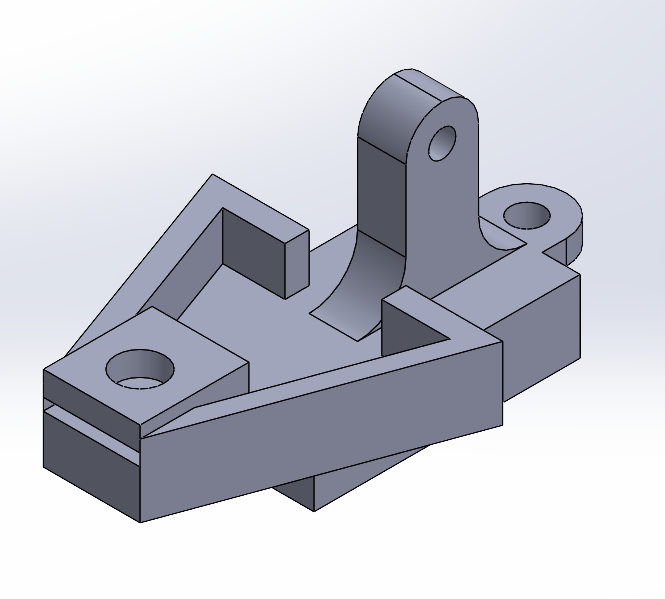
\includegraphics[width=0.7\textwidth]{src/figs/cad-and-dwgs/carriage-cad.png}
    \caption{Carriage}
    \label{cad:carriage}
\end{figure}

\begin{figure}[H]
    \centering
    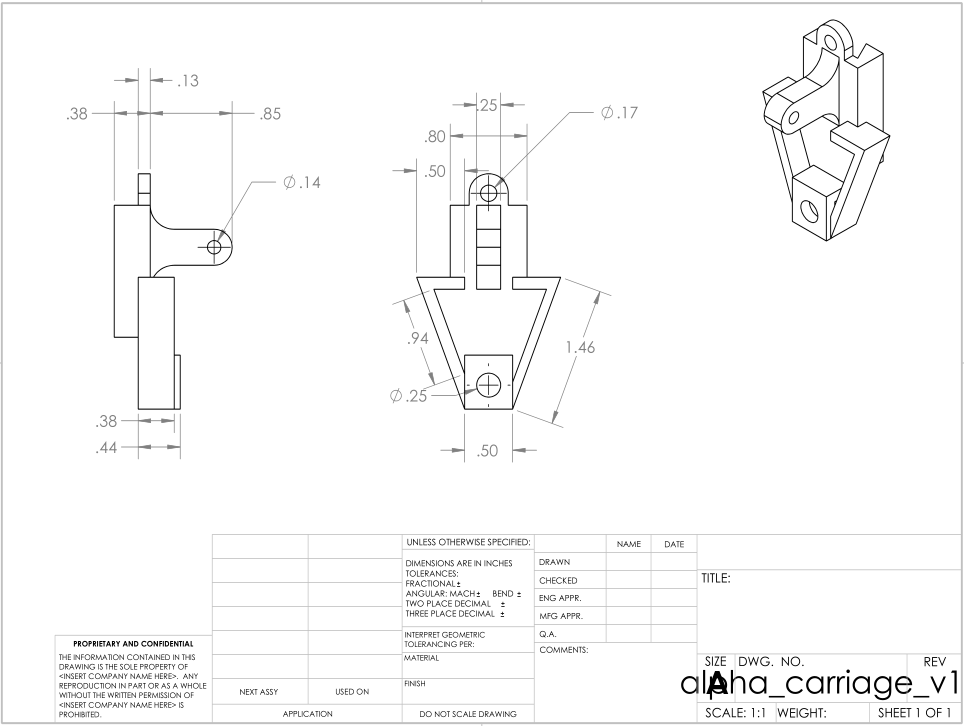
\includegraphics[width=\textwidth]{src/figs/cad-and-dwgs/carriage_dwg.png}
    \caption{Carriage drawing}
    \label{cad:carriage:dwg}
\end{figure}

\begin{figure}[H]
    \centering
    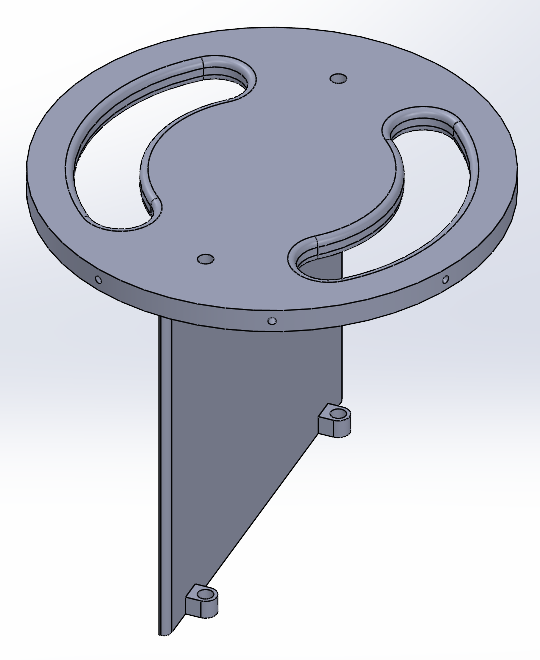
\includegraphics[width=0.7\textwidth]{src/figs/electronics_sled_base.png}
    \caption{Electronics sled base}
    \label{cad:electronics-sled-base}
\end{figure}

\begin{figure}[H]
    \centering
    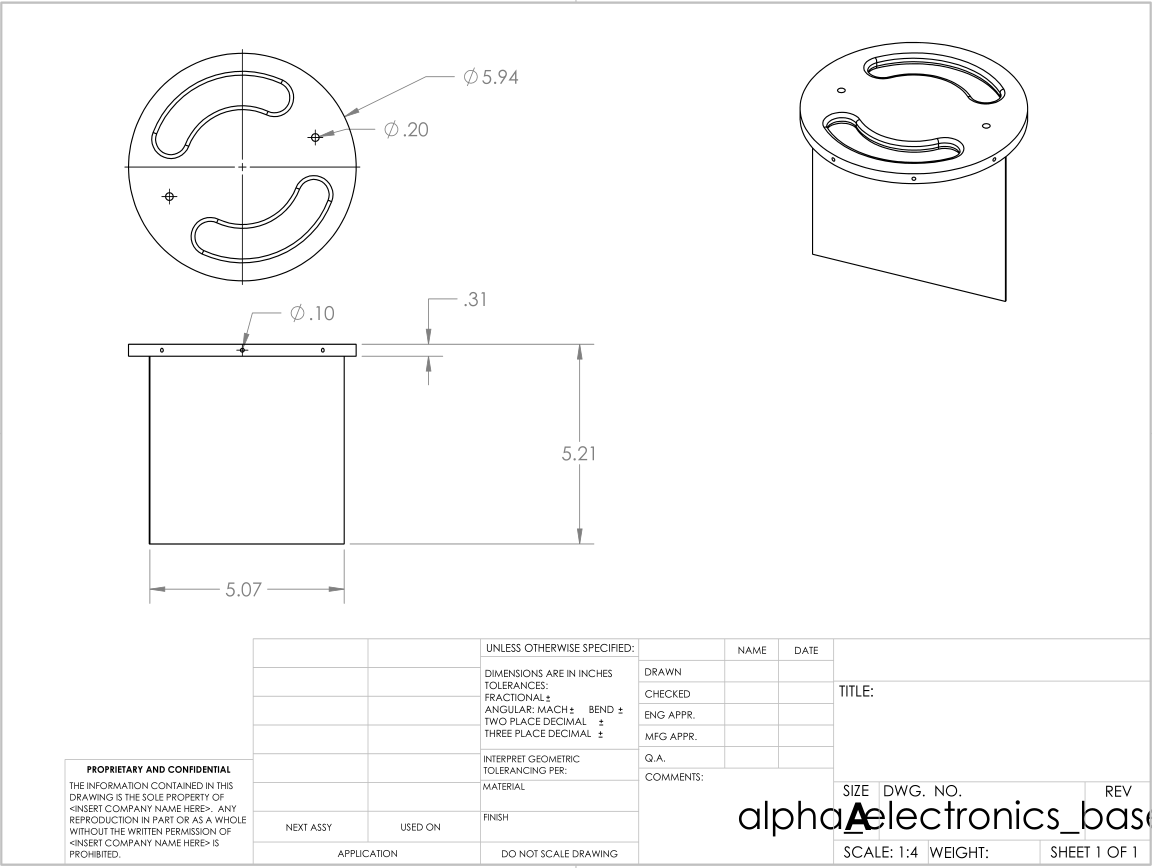
\includegraphics[width=\textwidth]{src/figs/cad-and-dwgs/electronics_base_dwg.png}
    \caption{Electronics sled base drawing}
    \label{cad:electronics-sled-base:dwg}
\end{figure}

\begin{figure}[H]
    \centering
    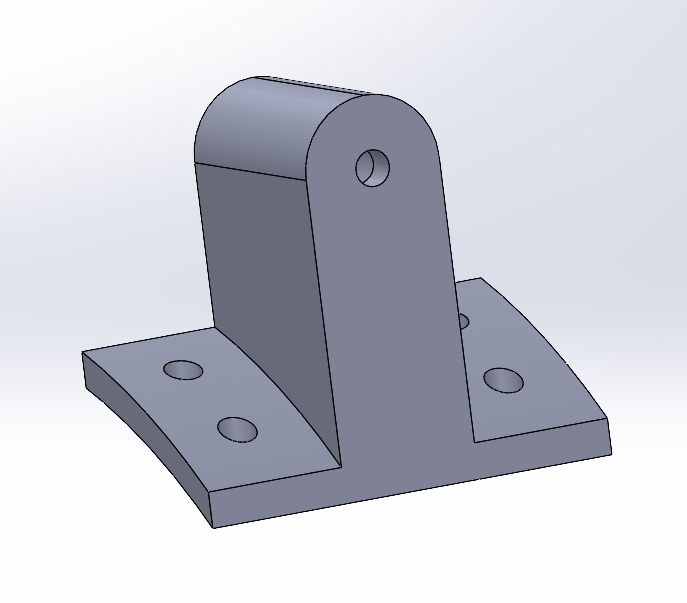
\includegraphics[width=0.7\textwidth]{src/figs/cad-and-dwgs/leg-pin-holder-cad.png}
    \caption{Leg pin holder}
    \label{cad:leg-pin-holder}
\end{figure}

\begin{figure}[H]
    \centering
    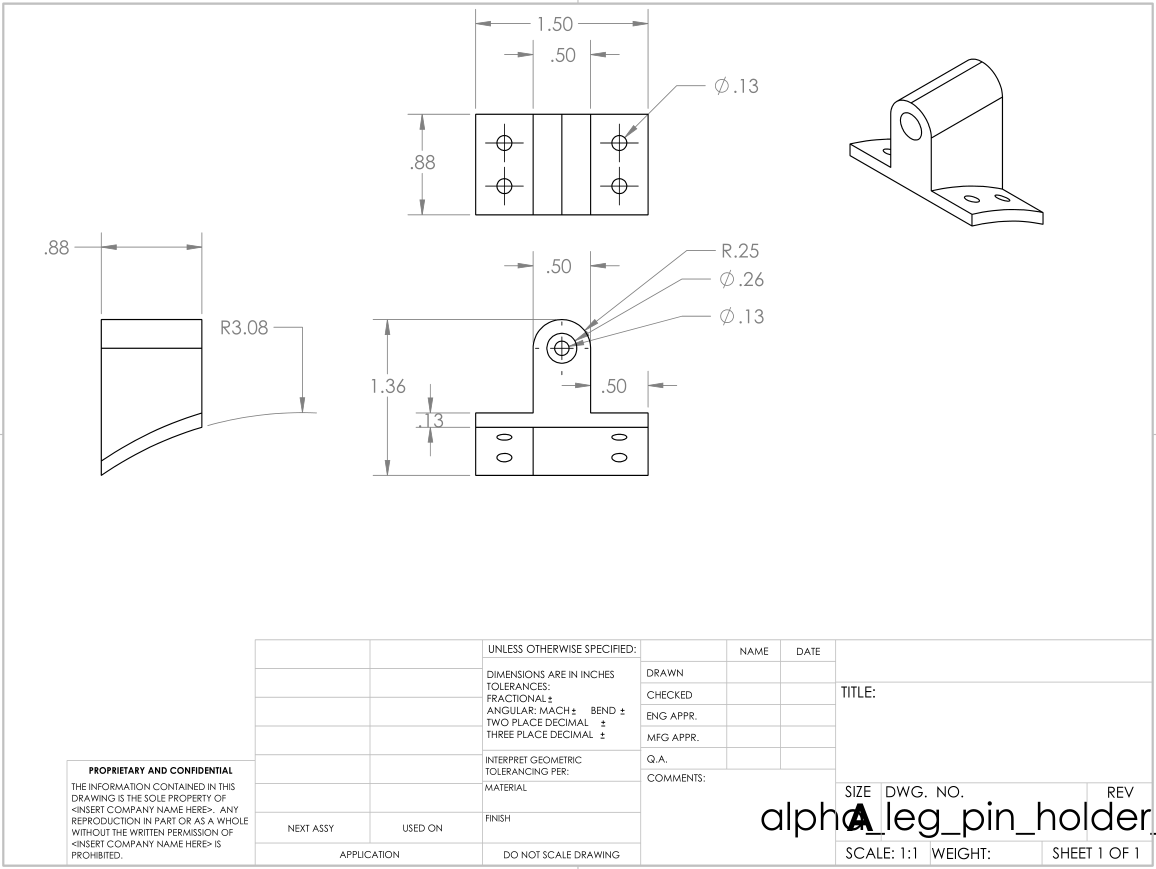
\includegraphics[width=\textwidth]{src/figs/cad-and-dwgs/leg_pin_holder_dwg.png}
    \caption{Leg pin holder drawing}
    \label{cad:leg-pin-holder:dwg}
\end{figure}

\begin{figure}[H]
    \centering
    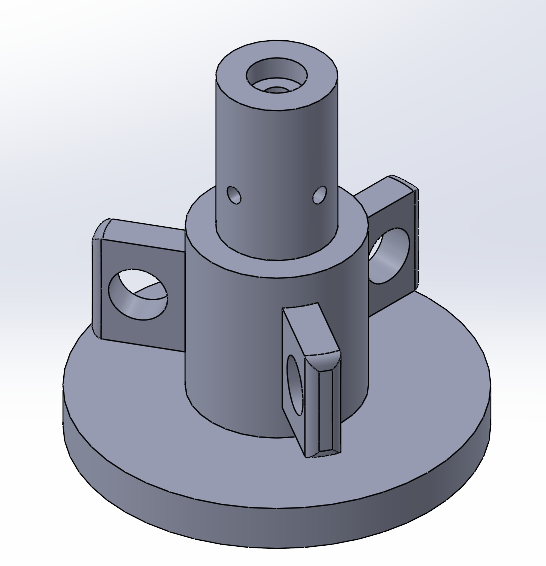
\includegraphics[width=0.7\textwidth]{src/figs/cad-and-dwgs/spool-cad.png}
    \caption{Spool}
    \label{cad:spool}
\end{figure}

\begin{figure}[H]
    \centering
    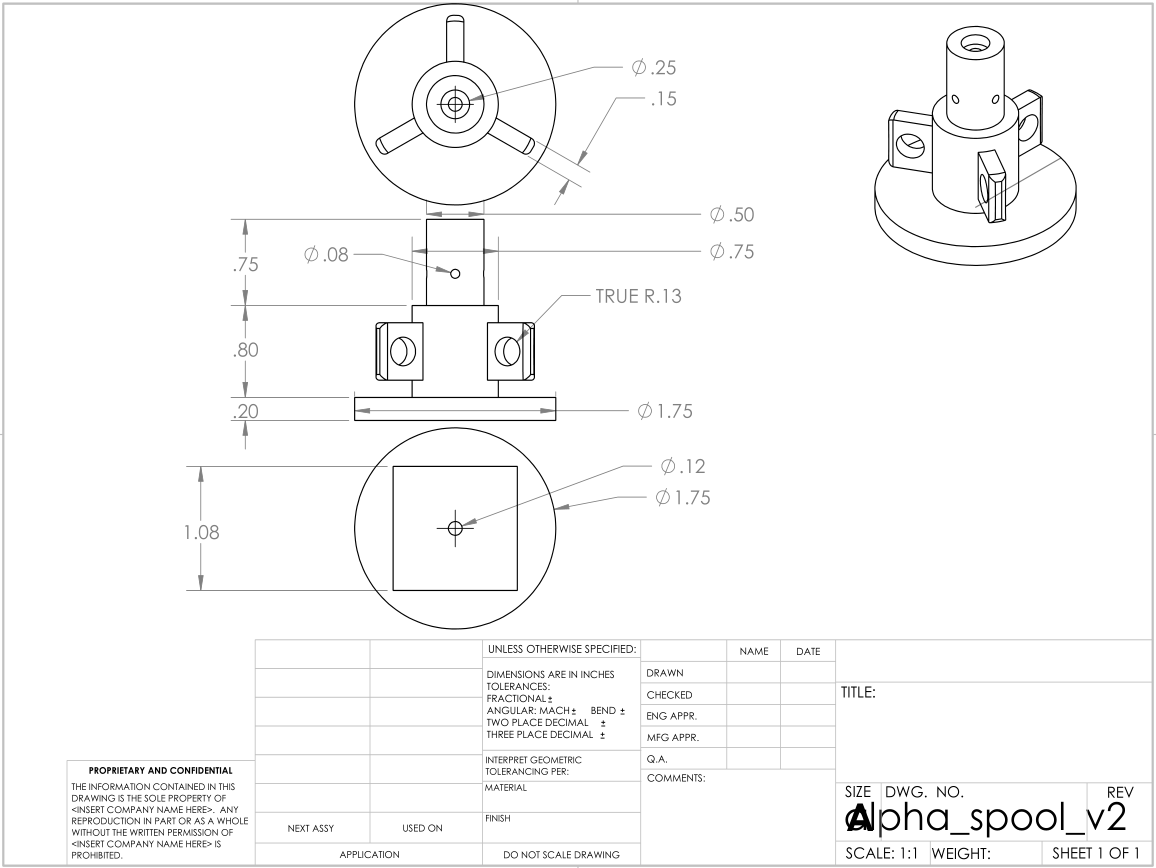
\includegraphics[width=\textwidth]{src/figs/cad-and-dwgs/spool_dwg.png}
    \caption{Spool drawing}
    \label{cad:spool:dwg}
\end{figure}


\begin{figure}[H]
    \centering
    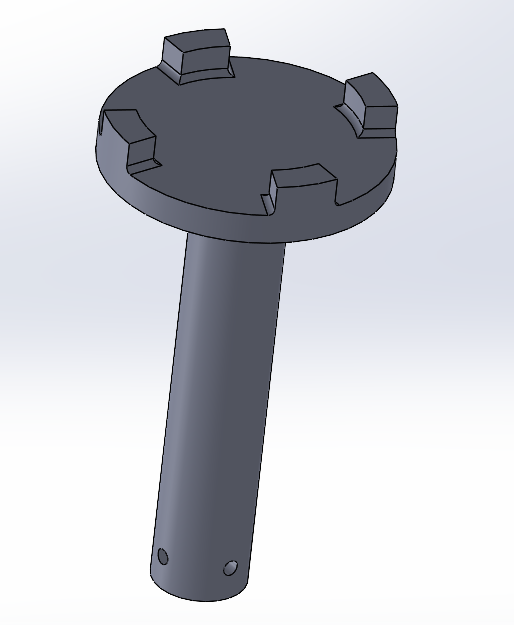
\includegraphics[width=0.7\textwidth]{src/figs/cad-and-dwgs/disk-cad.png}
    \caption{Arm locking disk}
    \label{cad:disk}
\end{figure}


\begin{figure}[H]
    \centering
    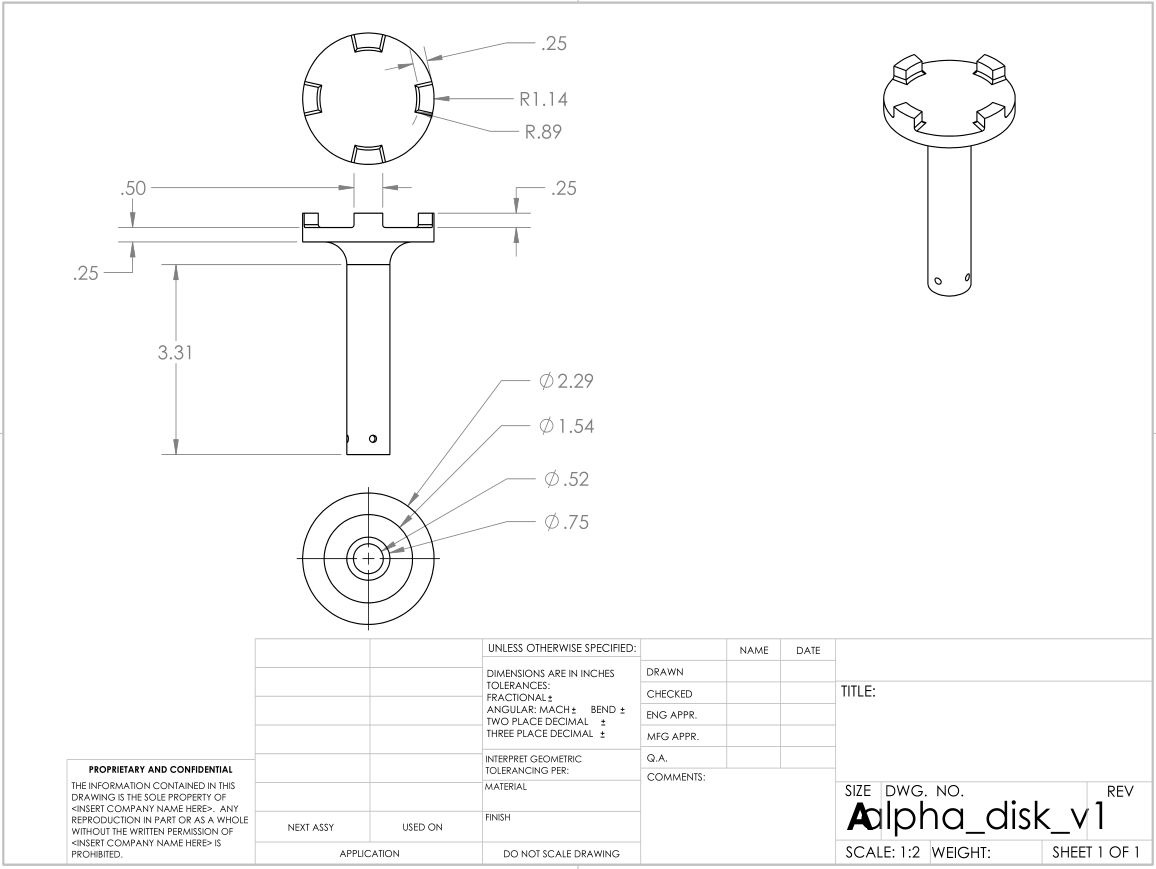
\includegraphics[width=\textwidth]{src/figs/cad-and-dwgs/disk_dwg.png}
    \caption{Arm locking disk drawing}
    \label{cad:disk:dwg}
\end{figure}

\begin{figure}[H]
    \centering
    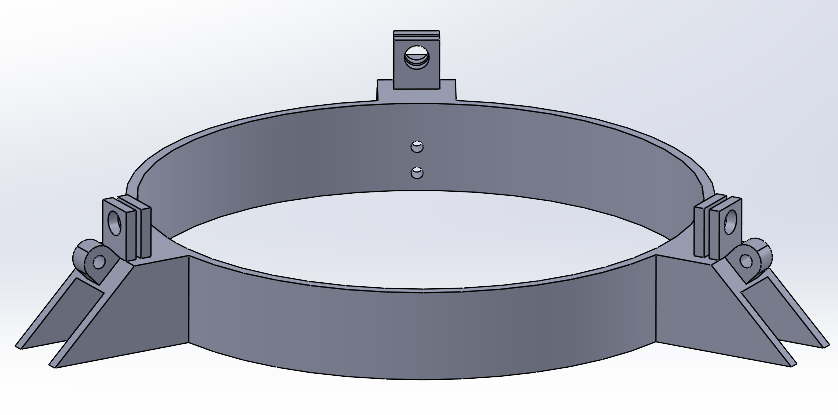
\includegraphics[width=0.7\textwidth]{src/figs/secondary-strut-support-cad.png}
    \caption{Secondary strut support}
    \label{cad:secondary-strut-support}
\end{figure}

\begin{figure}[H]
    \centering
    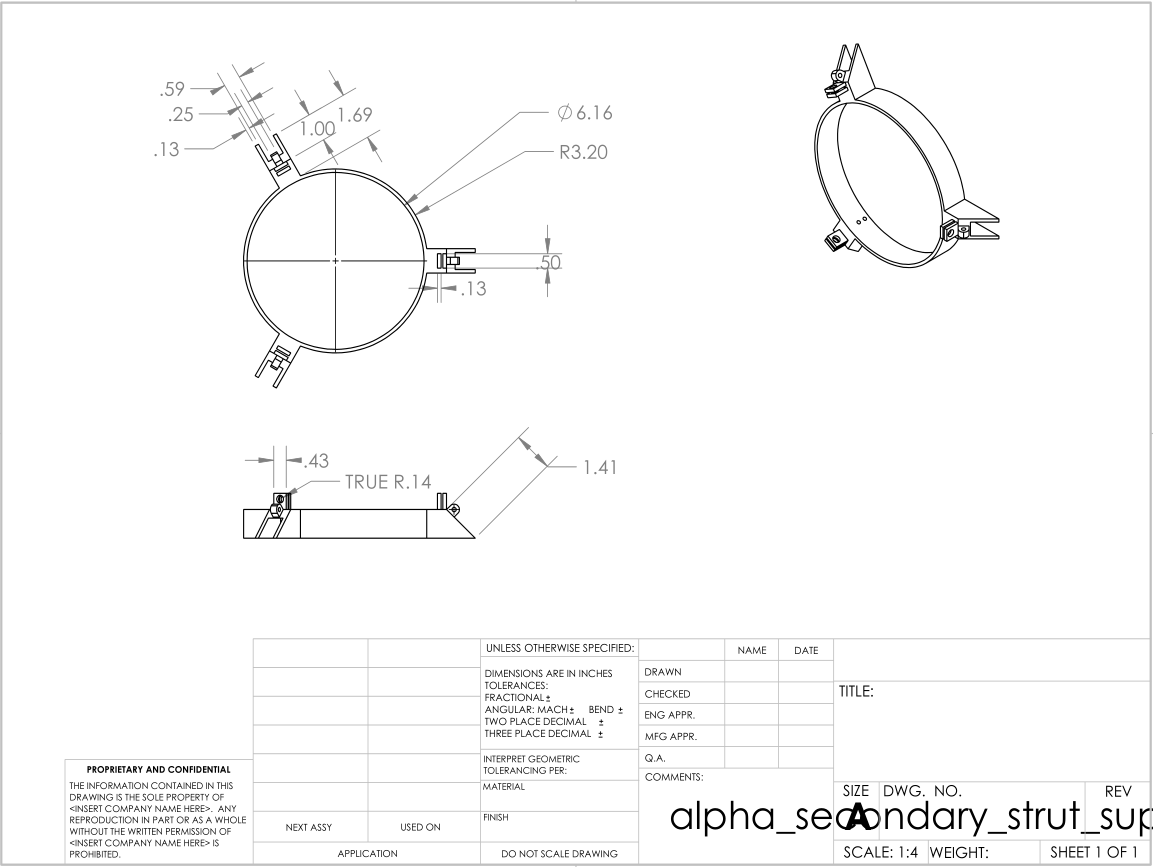
\includegraphics[width=\textwidth]{src/figs/cad-and-dwgs/secondary_strut_dwg.png}
    \caption{Secondary strut support drawing}
    \label{cad:secondary-strut-support:dwg}
\end{figure}

\begin{figure}[H]
    \centering
    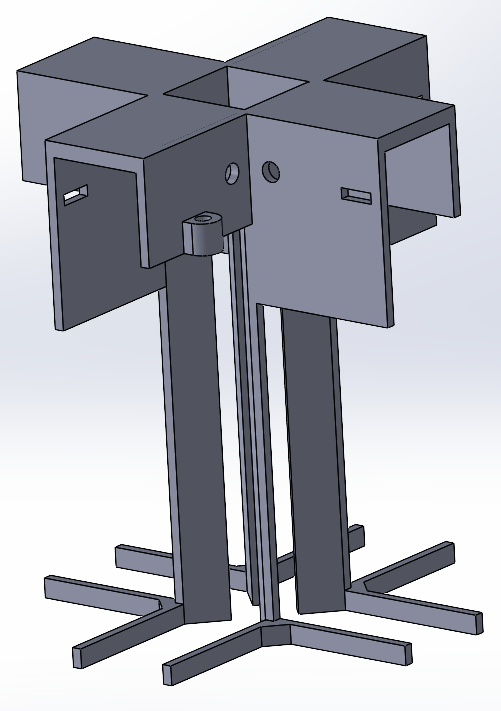
\includegraphics[width=0.7\textwidth]{src/figs/cad-and-dwgs/core-cad.png}
    \caption{Core}
    \label{cad:core}
\end{figure}

\begin{figure}[H]
    \centering
    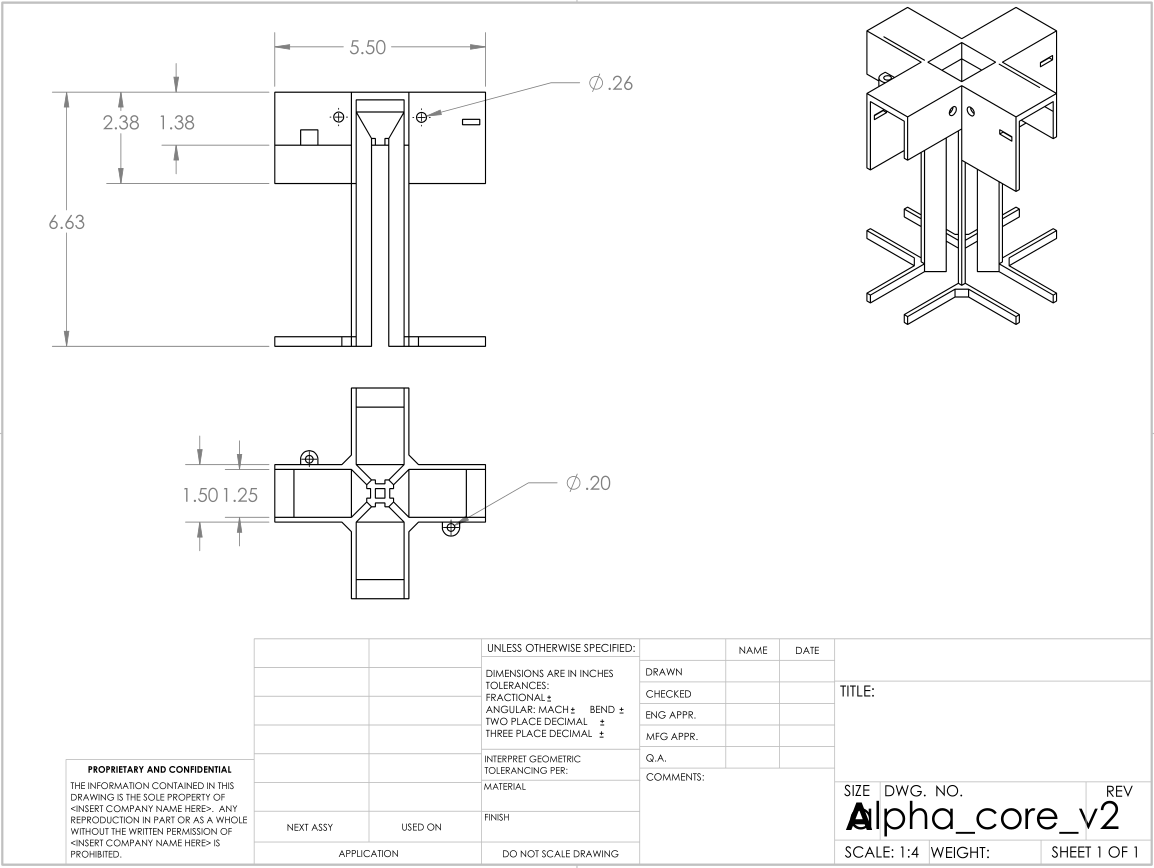
\includegraphics[width=\textwidth]{src/figs/cad-and-dwgs/core_dwg.png}
    \caption{Core drawing}
    \label{cad:core:dwg}
\end{figure}

\begin{figure}[H]
    \centering
    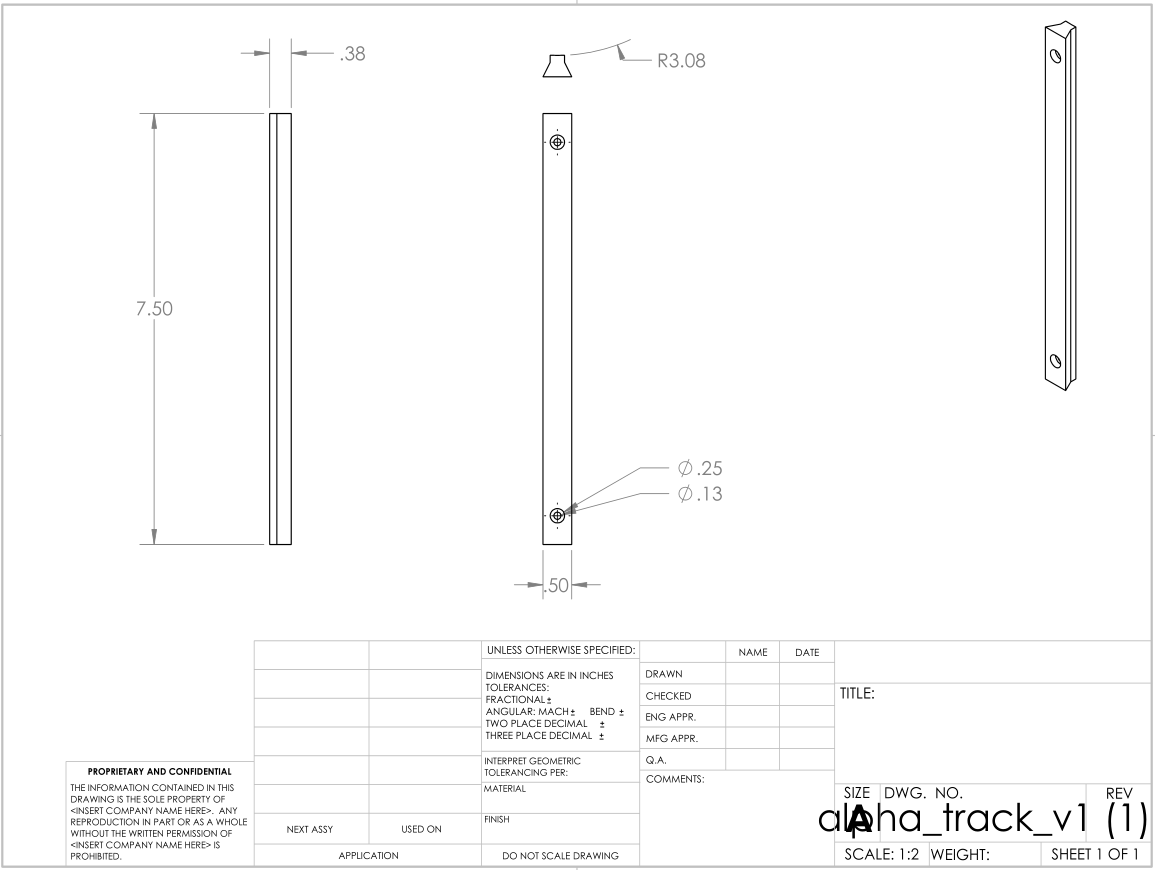
\includegraphics[width=\textwidth]{src/figs/cad-and-dwgs/track_dwg.png}
    \caption{Track drawing}
    \label{cad:track:dwg}
\end{figure}












\section{Controls and Electronics}
A basic diagram of the electronics wiring is shown in Figure \ref{cad:wiring} and a diagram showing the flow of signals/information between components is shown in Figure \ref{cad:signal-flow}.
\begin{figure}
    \centering
    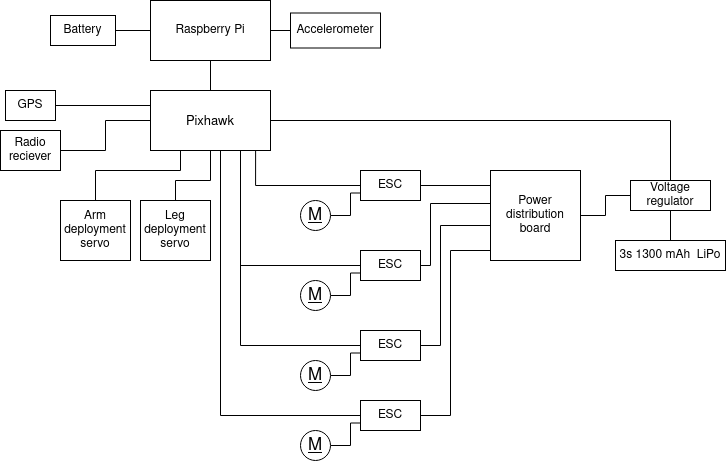
\includegraphics[width=\textwidth]{src/figs/electronics_wiring.png}
    \caption{Basic wiring diagram}
    \label{cad:wiring}
\end{figure}

\begin{figure}
    \centering
    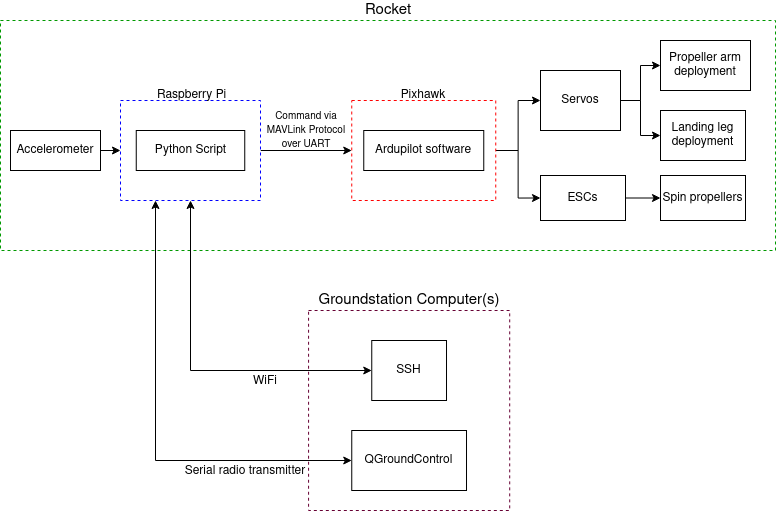
\includegraphics[width=\textwidth]{src/figs/signal_flow.png}
    \caption{Signal flow diagram}
    \label{cad:signal-flow}
\end{figure}
